\chapter{Microbial Community Analysis: Metagenomics and Metatranscriptomics}
\label{chapter:B}

\section{Introduction}
\subsection{Lake Washington Methane Cycling Studies}

The Lidstrom Lab has studied methanotrophic oxidation of methane in Lake Washington sediment for decades.
Methanotrophs are concentrated at the transition from aerobic to anaerobic soil.
This interface corresponds to both availability of methane, which rises from below, and oxygen from above \cite{lidstrom1984gradients, kuivilal1988, auman2000gradients}. %, which is required because methane is more reduced than biomass.
This microenvironment is rich in methanotrophs, methylothrophs, and other species.
When natural sediment samples are incubated in the lab with methane as the only food source, a high abundance of non-methanotrophs is often supported \cite{oshkin2015LW}.
Many of the abundant non-methanotrophs are methylotrophs, presumably consuming methanol, an intermediate of methane metabolism.
There are also many species which can only eat multi-carbon compounds, which must therefore consume excreted organic multi-carbon compounds, or cell biomass.
Trends in the types of communities that form in these sediment incubations have been observed  \cite{oshkin2015LW}.
Some species pairs appear to occur more than others.
Understanding the metabolic diversity of methanotrophs and methylotrophs in the sediment will advance understanding of why certain partnerships tend to occur, as well as understanding of a significant natural greenhouse gas mitigation system.

%Isolates first, but now new tools
% good resource: Methylotrophy in a Lake: from Metagenomics to Single-Organism Physiology https://www-ncbi-nlm-nih-gov.offcampus.lib.washington.edu/pmc/articles/PMC3147377/#B20
Early studies addressed these questions by sampling specific types of DNA from Lake Washington sediments (e.g. \cite{auman2002, costello2002, nercessian2005}), and studying isolates for which genome sequences were not available \cite{auman2000gradients, kalyuzhnaya2005Methylosarcina, kalyuzhnaya2006methylotenera}.
Later, significant laboratory efforts were used to isolate and sequence more species known to thrive in Lake Washington
    \cite{kalyuzhnaya2011isolates, beck2015isolates, mctaggart2015, kalyuzhnaya2015} to better understand these communities.
%These single species' metabolism can be further studied with transcriptomics and other tools (e.g. Chapter \ref{chapter:A}).
% (doesn't fit!) These strains can also be used as reference DNA for aligning shotgun sequencing reads.
%Furthermore, mixtures of small number of these pre-defined strains can be used to probe the potential of different partnerships and the underlying biology \cite{yu2016synthetic}.

% meta
Awareness that not all microbes can be isolated \cite{kaeberlein2002, stewart2012}, and that microbes probably behave differently when growing in communities due to influence of other microbes \cite{yu2016synthetic} motivates study of these microbes in their natural community compositions.
The omics studies used on single cultures (e.g. Chapter \ref{chapter:A}) can be applied to communities, though analysis becomes much more challenging.
When omics methods are applied to mixed populations of organisms, the prefix "meta" is applied, resulting in the terms such as  "metatranscriptomics".
Correspondingly the term "metagenomics" is used to describe sequencing the DNA of the community to allow inference of the abundant taxa and their genetic composition.
Having the paired metagenomic and transcriptomic data allows estimation of gene expression for those microbes, by mapping sequences to the reference DNA identified from the metagenomes.

\begin{figure}[H]
\centering
    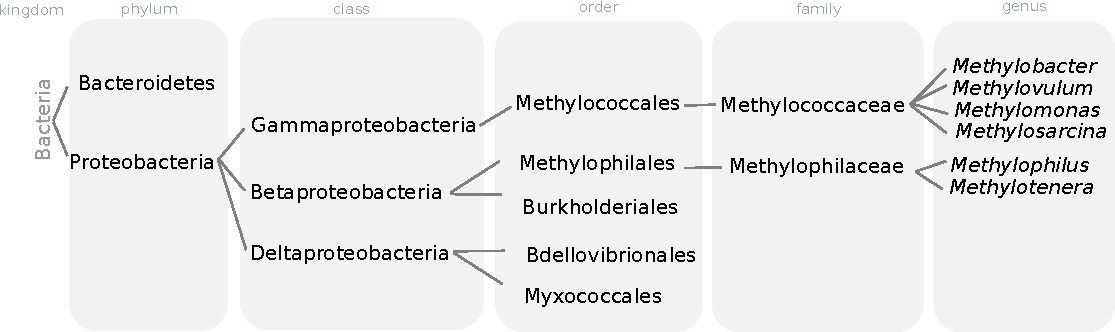
\includegraphics[width=1.0\textwidth]{./tex/chapter2/figures/170311_taxonomy_overview.pdf}
    \begin{singlespace}
    \caption[Taxonomy of microbes known to factor into methane oxidation in Lake Washington sediment.]{
       Taxonomy of microbes that often appear in methane incubations of Lake Washington sediment.
       The family Methylococcaceae is methanotrophic.
       The family Methylococcaceae includes non-methanotrophic methylotrophs.
       Burkholderiales grow on multi-carbon compounds, but in addition, some are methylotrophs.}
    \label{fig:taxonomy}
    \end{singlespace}
\end{figure}

Previous metagenomics and metatranscriptomics studies of Lake Washington sediment have highlighted dominance of the methanotrophic family Methylococcaceae \cite{beck2013LW, beck2014LW, oshkin2015LW, hernandez2015LW}.
These methanotrophs provide substrates for non-methanotrophic methylotrophs to grow \cite{beck2013LW}.
The particular methanotroph species and methylotroph species that dominate the sample is known to be influenced by oxygen availability \cite{hernandez2015LW}.
In previous studies, it was noted that low \ce{O2} tensions select for Methylotenera/Methylobacter partnerships whereas high \ce{O2} tensions select for Methylophilus/Methylosarcina partnerships \cite{hernandez2015LW}.
There is also a revolving cast of non-methylotrops including Burkholderiales and Bacteroidetes \cite{kalyuzhnaya2008Burkholderiales, beck2014LW}.
Better understanding of the metabolic roles that each of these species play, and why certain partnerships tend to form would provide insight into this greenhouse-gas mitigating microbial community.

\subsubsection{Goals of this study}
This study aims to identify the major methanotrophic, methylotrophic, and other microbial species that together enable methane consumption in Lake Washington, and deduce each taxa's contribution to the community metabolism.
Identification of which methanotrophs dominate in natural communities provides insights into how good past isolate studies reflect the true drivers of methane oxidation.
Identification of which metabolic pathways are expressed by these methanotrophs and the accompanying non-methanotrophs informs the mechanism of methane oxidation in this natural system.
Understanding each microbes contribution to the community metabolism allows hypotheses about genetic factors in methanotroph/methylotroph partnerships.

%For example, this study also aims to address the relative importance of two functionally redundant methanol dehydrogenase enzymes: Xox-MDH and Mxa-MDH. (cite).
%TODO: write more about this if I get results in the area.
%TODO: Some methylotrophs only have Xox.  So they are using it, or absent.

% --- How this dataset is poised to address these questions:    Experimental design: (don't make it too methodsy!)
The experimental design chosen to answer these questions is show in in Figure \ref{fig:experimental_design}.

\begin{figure}[H]
\centering
    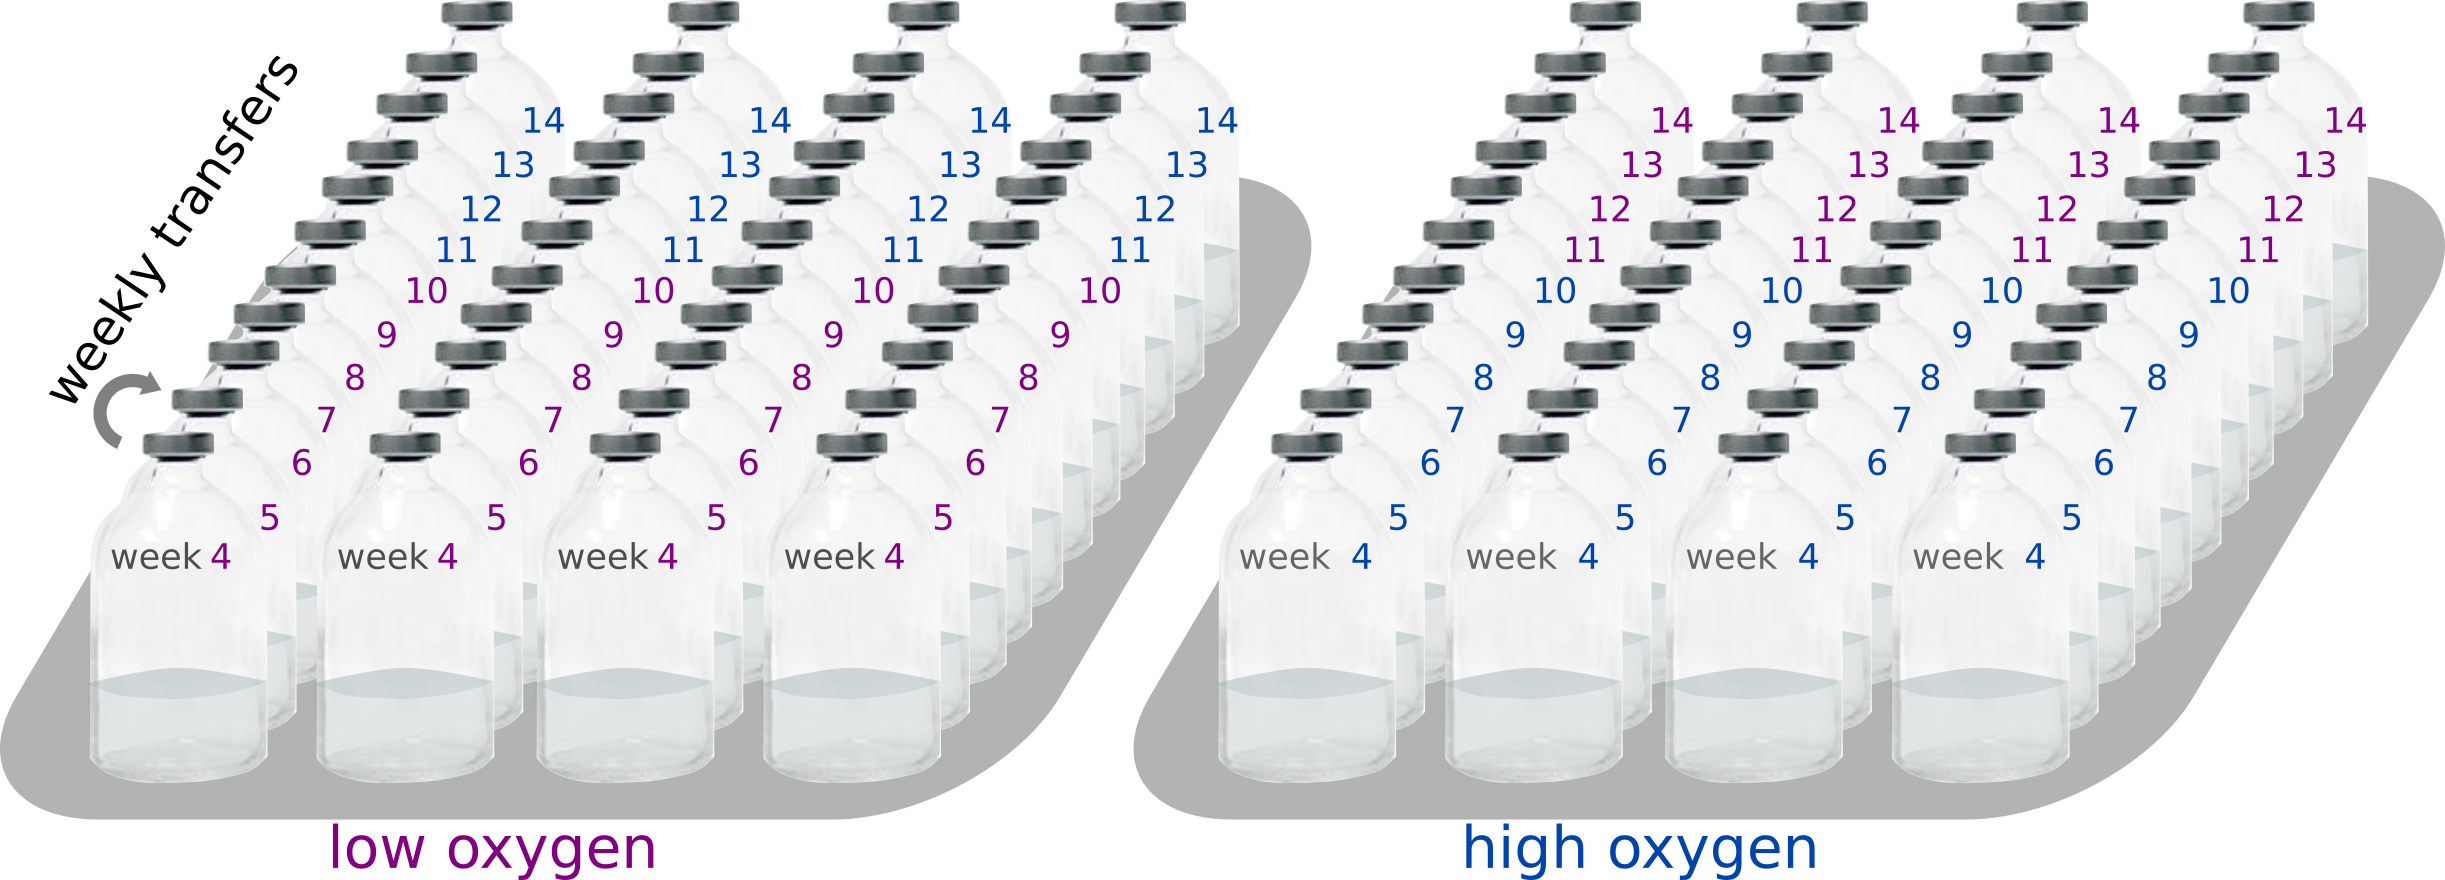
\includegraphics[width=1.0\textwidth]{./tex/chapter2/figures/170311_experimental_design_meta4--2_colors.png}
    \begin{singlespace}
    \caption[Experimental design.]{
       Sediment from Lake Washington, which had been thawed from -80$^o$C and cultured in 8 different bottles,
        half of which were treated with low oxygen, and half of which were at high oxygen (see methods).
	   Bottles were serially transferred for a total of 14 weeks.
	   The last four bottles in each series are at the opposite oxygen condition of the original experimental design
        (indicated by bottle label color switch).
	   Metagenomes and metatranscriptomes were obtained for weeks 4-14, resulting in 88 metagenomes and 88 metatranscriptomes.
	   }
    \label{fig:experimental_design}
    \end{singlespace}
\end{figure}

This relatively simple experimental design, including high degree of replication for studies of this type, was chosen to provide statistical power despite differences across replicates and measurement noise.
Variation across replicates can arise from stochasticity as communities rarefy, and are compounded by the noise-generating steps of nucleic acid extraction, ribosomal RNA removal (in the case of metatranscriptomics), library prep, and the sequencing process.
The most important environmental variable identified so in previous studies, the oxygen availability, was modulated while holding all other variables constant.
Availability of sequenced isolate strains from the very ecosystem enhance exploration of the dataset by providing some ground-truth biological facts.
Lake Washington isolates can also be integrated into positive controls for many of the computational methods.

% --- Data sets like this are rare and special.
Though sequencing has become routine in most biological domains, this dataset is exceptional for several reasons.
Having 4 replicates for each experimental condition is much greater than typical metagenomic studies.
Furthermore, most metagenomics/metatranscriptomics studies are single timepoint snapshots, rather than time-series.
Having 11 samples in each series leads to a total of 88 samples.
For each of the 88 samples, untargeted metagenomes and metatranscriptomes were gathered.
These pairs allow exploration of the community without the restriction of referencing cultured strains' genomes.
RNA was depleted, so the majority of our sequencing information is about expressed genes.
In all the dataset totals to 9TB, with approximately XX reads per sample.

% --- Insights into what's challenging
Despite the size and replication of this dataset, answering the questions outlined above proved challenging.
%There are many additional challenges in moving from pure-culture 'omics to meta-'omics, and these challenges were amplified by the large size of the data.
First, the study aims to answer who is there, without the luxury of using reference DNA to align sequencing data to.
Thus, the first task is to assemble reference DNA from the vast number of short sequences provided.
This DNA then becomes the basis for answering both "who is there", and "what are they doing".
Ideally, the assembly yields a small number of long sequences.
More often than not, however, under-sampling of DNA or lack of punctuation in well-sampled (highly abundant) strains leads to fragmented reference DNA.
This fractured reference DNA carries uncertainty and information loss through the rest of the analysis, so care must be taken to interpret all downstream results (discussed in Figure XX).

% -- Tool selection & evaluation is challenging.
Furthermore, tool selection and evaluation is challenging.
As discussed in the introduction, metagenomics and metatranscriptomics of natural microbial communities is a rapidly developing field laiden with methodological challenges.
For each step of inference, there are numerous tools utilizing different approaches one must choose from.
Given that each tool has different efficacy on different data sets, several tools are usually tried for each step.
For each tool, there are numerous tuning knobs the author encourages exploring, leading to a combinatiorial explosion of potential outcomes for each inference step.
The nearly complete turnover of tools approximately every 5 years leads to very few benchmarking studies, and review papers that are out date upon publication.
Benchmark studies comparing tools are rare and specific to a small number of data sets that may not behave like your own data set.
%Methods and metrics for tool evaluation are not standardized. repeated below

% --- Lack of standards in field
The field also lacks standards for assessing the efficacy of each inference step.
This is in part due to differences in goals across metagenomics/metatranscriptomics studies: some aim for high confidence inference about a specific sub-population such as a novel taxa, whereas others aim to describe the sample more broadly.
Many tools provide only limited insight into their efficacy on your particular dataset.
Care must be taken by the investigators to select the right tools, connect them properly, and evaluate results critically.
Often the trade-offs between tools are not evident until they are tested, and the data is explored with a critical eye.
Success in this field requires iteration as these insights are developed.

% --- So Big!
Furthermore, the size of this dataset is both a blessing and a curse
Yes, the high degree of replication and number of samples per series is essential for identifying hypotheses in noisy data.
However, many computational tools are not designed to scale to input data of our size, and fail when used on larger datasets than they were developed for.
While some fail quickly and with informative messages, other simply fail by running indefinitely without the tool either completing its task or aborting.
For some goals, the data can be broken into subsets, processed separately, and re-joined upon completion.
However, not every tool can operate on segments of the data, and extra care is required when stitching together results such that the next tool downstream is blind to such manipulations.
Despite the challenges, this thesis lays out preliminary results addressing both what microbes are present, and what they contribute metabolically.


%==========================================================================================================================================
%==========================================================================================================================================
%==========================================================================================================================================
\section{Metagenomics and Metatranscriptomics}

\subsection{Introduction to Metagenomics and Metatranscriptomic Inference}
Metagenomics and metatranscriptomics are umbrella terms for any project that uses sequencing of mixed populations of organisms.
It implies untargeted sampling of the samples' entire DNA or RNA pool, rather than selecting for specific types of sequences.
This is in contrast to 16S surveys, which amplify DNA from a segment of the conserved bacterial 16S ribosome \cite{kunin2008}.
Such sequences are used as a molecular clocks for large timescales, and allow for inference of the bacterial taxa present in samples.
16S studies do not allow the possibility to determine what genes each organism has available.
Sometimes two organisms are nearly identical at the 16S level, but have substantial metabolic differences due to insertions, deletions, and transposons.  % todo (cite) (tried for 20 min).
The term "metagenomics" is typically reserved for the un-targeted sampling of the entire community DNA pool.
Metagenomics affords the possibility of identifying the genetic composition of individual microbes, albeit after much greater analysis efforts.
Prior studies of Lake Washington painted the coarse 16S-based perspective of who is present in Lake Washington's sediment \cite{beck2013LW, hernandez2015LW, oshkin2015LW}, and did preliminary untargeted metagenomics \cite{beck2013LW, oshkin2015LW}.
This work focuses solely on untargeted metagenomics, to address the more challenging questions of microbial genetic composition, and to provide a basis for expression analysis.

%---- Isolates vs de-novo reference-free assemblies.
Once shotgun metagenomic samples are in hand, there are many possible ways to infer which organisms are present and what they express.
One approach is to assess how the samples relate to isolate organisms, by mapping to the reads to the isolates' genomes.
High mapping rates to an isolate genome suggests the sample contained a large abundance of a similar organism.
If their genomes are similar, mapping of RNA can inform the expression patterns of that organism in the sample.
This can afford an excellent benchmark for analysis of metagenomes or transcriptomes, but only if the isolate genomes accurately represent the strains and diversity of strains in the community sample.
However, isolates may often poor proxies for natural microbes given that the vast majority of isolates are not currently culturable \cite{kaeberlein2002, stewart2012}.
Even if the isolates are perfect proxies for some organisms, the set may be missing whole categories of other organisms.
This project did a preliminary study using isolate genomes as a reference for mapping metatranscriptome reads (Section XX), but discovered that a small fraction of the RNA mapped to the genes in the isolate genomes.
The project quickly pivoted to reference-genome-free workflows, whereby the metagenomic reads were assembled into contigs that collectively represent the DNA present in the dominant and semi-abundant microbes.
These contigs can be annotated to identify genes, and organised into genome bins intended to represent single strains or groups of highly similar strains.

\begin{figure}[H]
\centering
    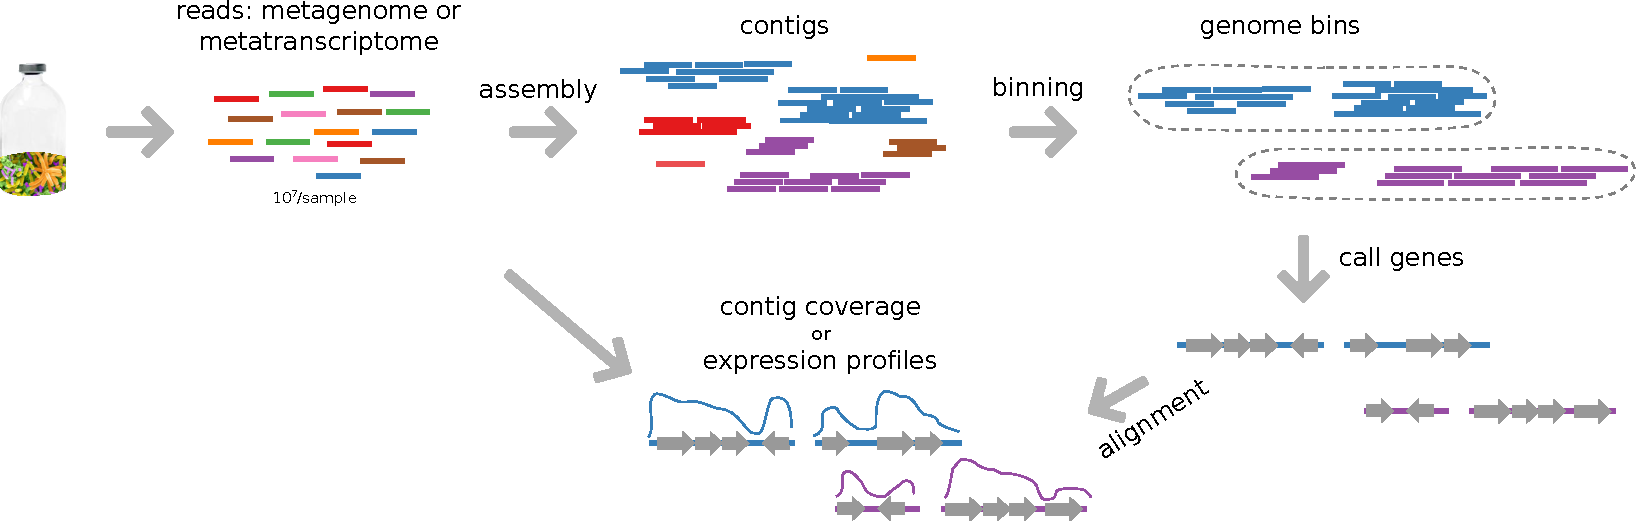
\includegraphics[width=1.0\textwidth]{./tex/chapter2/figures/170312_metagenomics_metatranscriptomics_overview.pdf}
    \begin{singlespace}
    \caption[Overview of metagenomics/metatranscriptomics workflow.]{
       Graphical introduction to basic vocabulary and inference steps of metagenomics and metatranscriptomics workflows.
	   Colored lines = single reads, long colored lines = contigs,
	   gray arrows on colored lines = gene calls, wiggly lines above contigs = coverage of alignment.}
    \label{fig:meta_workflow}
    \end{singlespace}
\end{figure}

The high-level representation of steps common to most shotgun metagenomics papers is shown in Figure \ref{fig:meta_workflow}.
The first step of reference-free metagenomics is assembly, wherein contigs are aligned and fragments are merged to infer the sequence from which the reads originated.
Binning aims to identify contigs that in aggregate represent single organisms, or groups of highly related organisms \cite{kunin2008}.
Genes can be called on the contigs, either before or after binning, to reveal the genetic potential of the parent organism.

The flow of information through metagenomics workflows can be thought of as liquid flow through piping with leaks.
Each software step can be though of as a pipe.
Flow (read accountability) can be measured at the input and exit of pipes (represented by flow gauges), allowing identification of how well output data reflects the original samples, and at which step(s) information was lost.

\begin{figure}[H]
\centering
    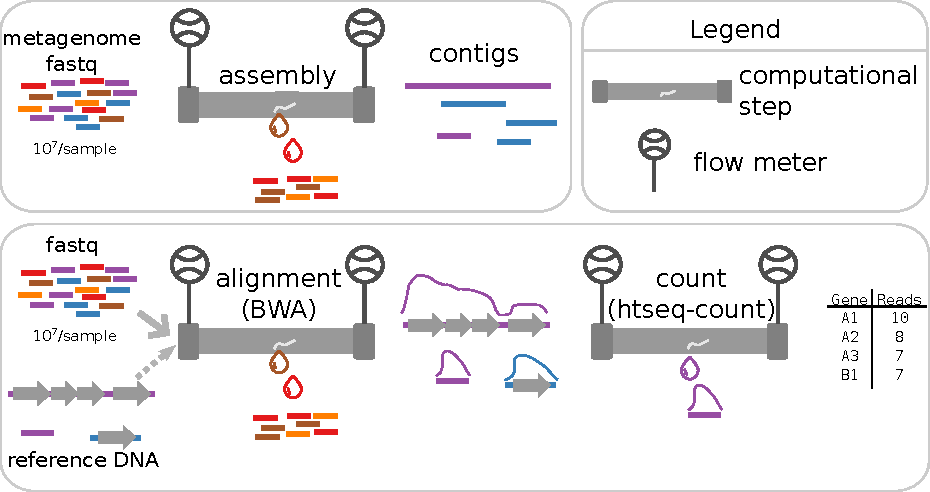
\includegraphics[width=0.8\textwidth]{./tex/chapter2/figures/170312_pipe_leaks.pdf}
    \begin{singlespace}
    \caption[Framework for assessing information loss in workflow steps.]{
        Cartoon representing the ability to deduce information loss at different steps of the metagenome/metatranscriptome workflow.}
    \label{fig:pipe_leaks}
    \end{singlespace}
\end{figure}

%---- Pipe description
A simplified cartoon of the framework used to assess efficacy of each tool in the workflow is illustrated by Figure \ref{fig:pipe_leaks}.
For papers where the goal is to describe one or several novel organism(s) with high confidence (cite), the loss of information (reads) along the way may not be a significant concern.
Often papers in this category do not clearly report an estimate of that organisms abundance in the natural community.
% Don't trash other papers \cite{evans2015} , or obscure absolute abundances by using relative abundances \cite{daly2016}.
Other papers try to describe a more holistic description of the community \cite{kantor2017} by describing the diversity of organisms found in bins from the sample.
In this case, it is crucial to quantify what fraction of the original sample is described by the output of your analysis.
These statistics are usually not stated clearly, allowing readers to over-estimate the importance of the described taxa in the real ecosystem.
% At this stage, or research is in this camp, and the result section will highlight how this frame of mind guided selection of tools.
The pipe analysis framework illustrates the approach of this paper: use multiple monitoring methods to determine which pipeline steps are associated with information loss.
These statistics are reported throughout to prevent misinterpretation of claims about the community compositions and expression patterns.
%This thesis aims to describe the community holistically, and thus strives to clearly report assembly, binning, and read mapping effacy so as to not overstate claims or exaggerate community simplicity.
% Many literature studies report small and incomplete descriptions about efficacy of their assembly and binning, which obfuscates leaks in the analysis pipeline and corresponds to over-simplified descriptions of the environment under study.  % Don't cite: hard to be ceratin I read carefully enough to call out papers by name.  It's also not nice!

%----- There is no road map!
Each arrow can be executed by several or sometimes dozens of competing software packages \cite{sangwan2016,thomas2012}.
Each tool can report basic statistics about efficacy based on inputs and outputs, but it it up to the researcher with larger-scope understanding of the project goals to write scripts to critically assess efficacy of the tools in aggregate.
Results from one software package can give you better insight about how to evaluate the other packages' results, so an iterative process with various somewhat-equivalent tools can maximize the accuracy of your results.
Finally, more data is great for software tools trying to extract information from uncertain data, but many tools are not designed to work on sequencing data as large as this one.
%Tools choke.  Just don't complete.
Sometimes the parameters can be altered, sometimes you can break up a dataset and feed it to a tool in pieces, but sometimes the size is a deal breaker.
It is the role of the computational biologist to learn enough about the competing tools to select a handful to try, develop metrics and priorities for the trade-offs of each tool, project complex data into summary graphs, and decide which tool is the best fit for the research goals.

\subsubsection{Assembly}
%---- Why assemble
Analysis of metagenomic and metatranscriptomic data usually beings with assembling metagenome reads into contigs (Fig \ref{fig:meta_workflow}), which are contiguous length of genomic sequence in which the order of bases is known to a high confidence level. %(JGI)
The metagenomes can be aligned to these contigs to infer the abundance of organisms.
The transcriptomes can be aligned to these same contigs to infer what genes are expressed.
In principle, metagenomes and metatranscriptomes can be aligned to isolate genomes rather than contigs, however, in practice meta-omics experiments are used precisely when the isolates available are known to be incomplete representatives of the microbial community under study.
Even if a similar organism has been isolated, the investigation may be probing the diversity of similar organisms, or the influence of less abundant microbes on the community's function.

%---- Not all assemblies are created equal
The challenge of assembly scales with the complexity of the microbial community.
High species diversity and strain-level heterogeneity add challenge to assembly \cite{kunin2008, thomas2012}.
Communities with a small number of well-delineated species tend to assemble better, yielding shorter numbers of long contigs.
In contrast, complex communities' high diversity can lead to assemblies with fewer long contigs and more short contigs \cite{kunin2008}.
These shorter contigs are more challenging to analyze and can lead to an incomplete portrait of a community.
Short contigs' are more difficult to call genes on, and are also more difficult to bin because measures like GC and differential abundance are noisier for short contigs than long ones \cite{sangwan2016}.
The most common measures of assembly efficacy are characteristics of the contigs themselves.  How many are there?  What is the length of the median contig (termed "N50")?
This thesis advocates for an additional measure not seen in other published work: the fraction of the original reads that map to the assembled contigs.   % todo: "seldom seen" instead of "not seen"?
% Dont' talk about restricting to contigs > 1.5kb.

\subsection{Elviz Assemblies}
%---- JGI assemblies
Many sequencing projects including this one are done by the Joint Genome Institute (JGI), which provides some bioinformatics processing in addition to providing un-processed reads.
The software they run assembles contigs for each sample individually, predicts genes, and calls taxonomy for contigs \cite{cantor2015}.
They also report the number of reads and average coverage for each contig.
These measures are a great starting point for answering "who's there" in terms of taxa abundance, but does neglect information about reads that did not assemble well and thus must be used with caution.

%---- Not assembled together
The contigs JGI provides are assembled for each sample, individually.
Thus the contigs are not shared across samples, and comparison across samples is hindered.
For example, it is difficult to infer whether a particular gene is expressed differently in two samples if the contigs used as reference DNA are not the same across samples.
More powerful analyses can be done when the DNA from all metagenomic samples are assembled at once.
This makes it possible to get a table of gene expression that is comparable across samples.
Such an assembly also leads to more powerful binning (discussed below) by providing extra features to cluster with: the differential abundances of each contig across the n samples \cite{albertsen2013}.
Since the number of reads originating from a particular organism should be proportional to its abundance, the DNA coverage for a set of contigs originating from an organism should be similar in a particular sample, and correlated across samples.
The per-sample nature of the JGI contigs drove the types of analyses that data was used for, and motivated generation of co-assembled contigs to represent the entirety of the dataset as discussed below.

\subsubsection{Binning}
%---- Definition & Why
Desire for understanding at organism-level often leads investigators to approximate genomes as best they can from a set of metagenomic contigs.
The phrase "genome bin", often called simply "bin", is used to describe a collection of contigs used to approximate a single organism's genome.
"Bin" implies the collection is expected to be somewhat incomplete and potentially contaminated by DNA of other strains or species.
Bins allow inference of which metabolic pathways are available, and can be used as a reference to map RNA to for quantification of how these genes are expressed.
Higher confidence claims would be possible upon isolation of the organism represented by the genome bin, but laboratory isolates are often not obtainable either due to obligate partnerships with other organisms, or a variety of intolerances to laboratory conditions \cite{stewart2012}.
Binning can be done before or after annotating genes on the contigs, as very few methods use gene calls in the binning process (cite?).

%---- Overview of binning tools' strategies
The most common features used to bin contigs include contig GC content, tetranucleotide frequency, other oligonucleotide frequencies, and differential abundance across samples \cite{sangwan2016}.
Most aim to be effective without needing reference genomes to align to.
% can't find citation for using an isolate as a binning reference.  Only for assembly.  Drop??

%---- Rarefaction, species heterogeneity
The ability to get clean genome bins varies wildly from project to project.
As with assembly, more rarefied samples with low levels of strain heterogeneity are more amenable to binning \cite{kunin2008, thomas2012}, as the contigs are more likely to be long and few in number.
Longer contigs have reduced noise for measurements of GC ratio, tetranucleotide freq, and differential abundance \cite{sangwan2016}.
This in turn leads to less ambiguity when sorting contigs into respective bins.

%---- Bin assessment
The quality of bins can be determined by combining metrics of completeness, contamination, and efficacy of representing the sample.
Completeness and contamination checks can be automated by use of CheckM \cite{parks2015}, which uses the presence of marker genes in each bin as the basis for its approximations.
The marker genes used by CheckM are different based on the approximate taxonomy CheckM approximates for the bins.
While this is certainly more effective than one set of genes used for all microbes, the reference sets available may not be good fits for the particular microbes under study.
Furthermore, the choice of reference gene set might be poor for messy bins that  contain contigs from wildly different taxa.
Some papers determine completeness and contamination by manual inspection using domain-specific marker gene sets (cite).
For papers published before CheckM, this was the best option, however CheckM does allow the possibility of adding custom marker gene sets to their analysis pipeline.

%---- Binning tools
The three tools used herein combine sequence composition and coverage across multiple samples as inputs to machine learning algorithms to automatically cluster contigs into genomes.
The differences in their algorithms are only vaguely described in the literature and, differences in their output characteristics are seldomly reported \cite{sangwan2016}.
Metabat \cite{metabat2015} uses k-medoid clustering of a distance measure composed of tetranucleotide frequency and abundance.
% ** doesn't use marker genes **
MyCC \cite{mycc2016} uses affinity propagation to cluster contigs, and uses the presence of marker genes to correct clusters.
%"an automated binning tool that combines genomic signatures, marker genes and optional contig coverages within one or multiple samples"
%"FetchMG extracts 40 universal phylogenetic marker genes"
%"AP-generated clusters were finally corrected based on the sequences harboring marker genes"
CONCOCT \cite{concoct2014} uses a Gaussian mixture model fit with a variational Bayesian approximation, on features thinned out via principle components analysis (PCA).
% This says it uses marker genes, but the original paper doesn't mention it.
% Manual curation
Almost every high-quality bin published in high-profile papers has used tools such as these, but is subsequently refined by manual curation, with methods only vaguely described.

\subsubsection{Mapping RNA}
Metatranscriptomes can be mapped to contigs or bins.
A key variable to consider is what you want to happen with reads that map to multiple places.
If a read maps equally well to two different contigs in a bin, should it be randomly assigned to one locus, or thrown away?
If the study is aiming for differential expression type analysis, than the latter is better.
Discarding ambiguous reads is the default of most alignment and counting tools.
If the study aims instead to describe a holistic picture of expression in a sample, it may be worth guessing the source of the DNA, which will certainly be wrong some of the time.


%==========================================================================================================================================
%==========================================================================================================================================
%==========================================================================================================================================
\section{Methods}

\subsubsection{Experimental}  % Note that work was done previously, so I'm not implying I did it.
The culturing and sample preparation was done by Maria Hernandez, a visiting scholar.
Sediment stored in DMSO on previous sampling trip was thawed from -80$^o$C and distributed into 250 mL bottles containing 50mL of NMS medium \ref{fig:experimental_design}.
Samples started with XX amt of methane (XX mL), and either low oxygen (XX amt) or high oxygen (XX).
Bottles were serially transfered for 14 weeks.
The bottles were kept sealed (air-tight) between serial transfers; the gaseous compositions for the days between transfers were not measured.
Bottles were shakedn at XX RPM and held at XX degrees.
Metagenomes and metatranscriptomes were obtained for all samples corresponding to weeks 4-14.
Earlier weeks were omitted due to potential effects of residual DMSO, and interest in prioritizing sequencing of later, more-rarefied samples.
The oxygen conditions (low/high) were switched for the last 4 bottles in each series (see Figure \ref{fig:experimental_design}).

\subsubsection{Sequencing}
This large dataset was made possible by a Joint Genome Institute sequencing grant (cite the \#? XX).
JGI sequenced all samples on an Illumina platform to produce the 88 metagenomes and 88 metatranscriptomes.
Ribosomal RNA was removed before sequencing the metatranscriptomes.
%~ XX (?? Paired ended?) reads per sample, for both metagenomes and metatranscriptomes (??).

\subsubsection{Elviz Analysis}
Along with raw sequencing outputs (fastq.gz files) for each sample, Elviz data was provided \cite{cantor2015}.
These data included one assembly per metagenome, corresponding contig statistics, and transcriptome alignment statistics.
In addition, they provide taxonomy for each contig, to some degree of certainty: some contigs' taxonomy stops at family, while others are specified to the genus level.
The taxonomy, contig lengths, and number of reads mapped to each contig were used to infer the distribution of taxa in each sample.
The metric used was the fraction of reads assigned to contigs with the specified taxonomy (\url{https://github.com/JanetMatsen/elvizAnalysis/blob/master/abundance_utils.py}).
Length of contigs was not normalized out, or the abundance of short contigs would dominate the results.
The code checks that each samples' abundance summed to 1.

Tools were written to aggregate (a) based on taxonomy level, or (b) everything below a taxonomy level.
Contigs with taxonomy not desired to the specified level were grouped into "other".
This framework was also used to summarize abundances at mixed taxonomy level (e.g. phylum Bacteroidetes, order Burkholderiales, family Methylococcales, and family Methylophilales) \url{https://github.com/JanetMatsen/elvizAnalysis/blob/master/abundance_plot_utils.py}.

Statistics for the 88 samples were merged with information about the oxygen, replicate, and week values corresponding to each sample using Python and Pandas.
Plotting was done with seaborn.

\subsubsection{Computational resources}
This computationally-intensive research was supported by research grant, which included \$XX and expert consulting on how to best utilize the vast services offered.
AWS allows per-hour rental of machines with different specifications, that the user can choose based on algorithm needs.
Furthermore, the ability to share machine images greatly facilitates the potential reproducibility of research.
Upon project completion, we will provide access to an AMI and allow others to re-run our analyses.

The machine ("instance") type used in all methods to follow was an AWS c4.8xlarge instance, which has 36 cores, and 60GB memory.
This was sufficient for all work, other than the memory-intensive assembly step, as noted below.
Instances could be turned on and off as needed, reducing compute cost.
This is in contrast to sharing a similar machine with the entire Beck Lab, which would have slowed down analysis and caused conflicts when certain computations used all of the compute resources, sometimes causing computer failure.

Each instance obtained data and wrote results to a shared file system
The 9 TB of data, scripts, and results were stored using the AWS Elastic File System (EFS).
EFS is AWS's most versatile and highest performance (most expensive) file storage, which allows you to have multiple instances reading/writing to the same directory.
This shared nature of the files allows the user to spin up a second computer instance as needed, and read/write the exact same set of files.

%---- Computation parallelization
Parallelization of compute tasks was done by splitting jobs across a single large computer, or across separate EC2 instances.
When tasks were parallelized across one powerful computer was done with Gnu parallel or Python's pool.map.
When parallelizing across more, often weaker, computers, an AMI was made that mounts the EFS-stored data.
These instances were usually started by hand through the console, though proof of principle studies using the Amazon Command Line Interface (CLI),
    and an Autoscaling/SQS service pair were explored to set the foundation of future work (see repository XX) for the templates developed.

\subsubsection{Map to isolate genomes}
As a preliminary study, the metatranscriptomes were mapped to 55 genomes isolated from Lake Washington by the Lidstrom lab.
The sequences were downloaded from NCBI, and concatenated together before mapping.
Mapping to the multi-fasta rather than the individual genomes prevents double-counting of reads that map well to multiple loci.
BWA-mem \cite{li2009} with default settings was used to map each transcriptome to the multi-fasta, and htseq-count \cite{anders2014} was used to tabulate expression estimates.
Samtools \cite{li2009samtools} was used to evaluate mappings by BWA.
Note: the default of BWA is to flag reads that map equally well to two or more loci as having quality score 0; these reads are then not included in the tabulated results by gene-name.
This is the best-practice approach when doing differential abundance analysis, but does lead to under-estimation of gene expression levels and lower accountability of the original fastq reads. % TODO: cite

\subsubsection{Assembly} % (Dave)
Assembly to produce contigs was done on pooled quality-trimmed metagenome reads via Megahit \cite{li2015}.
This memory-intensive computation was done on an AWS instance with 1 TB of memory.
Assembling of multiple samples simultaneously provides a shared set of contigs to use when mapping DNA reads or RNA-seq reads from any of the 88 samples.
This in turn allows for comparison of gene expression across samples.
The fraction of reads represented by the assembly, in aggregate, were measured to verify assembly efficacy.
%Tune knobs until …
%Followed protocol ...

\subsubsection{Gene calls}
Genes were called on contigs with length greater than or equal to 1.5kb using Prokka \cite{seemann2014}.
This was cutoff was selected because shorter contigs are not recommended for inclusion by most binning tools documentation.
Additionally, shorter contigs are less likely to have genes identified on them, as genes are more likely to be incomplete due to the edges.
Prokka did not tolerate an input size of the scale, so the input fasta was broken into 5 files of approximately equal size.
These were processed in parallel, using Python's pool.map function.
A \href{https://github.com/BeckResearchLab/meta4/blob/master/m4b_binning/assembly/prokka/contigs/glue_together_gffs.py}{script} was written to merge the resulting annotated general feature format files (.gff files) into one representing all contigs $\geq$ 5kb.

\subsubsection{Checking contigs' ability to represent each metagenome}
The loss of information resulting from omitting short contigs was assessed by counting the number of reads that map to contigs $geq$ 1.5kb, and comparing that to the total number in the raw metagenome fastq.gz files.
This represents an upper bound in information content for the assembly step.
Again, this used BWA \cite{li2009}, and a \href{https://github.com/BeckResearchLab/meta4/blob/master/m4b_binning/assembly/data/sample_info/count_reads_in_each_sample.sh}{script} written to count raw fastq reads.
Pandas (Python) was used to merge results together.

\subsection{RNA-seq: mapping to contigs $\geq$ 1.5 kb}
Like all other mappings, transcriptomes were mapped with BWA-mem (default settings), and per-gene results were summarized with htseq-count.
Contigs $\geq$ 1.5kb were used as reference DNA.
Metatranscriptomes were mapped to these contigs all at once, rather than to each bin individually in order to reduce over-counting.
This does result in reads mapping identically well to two places being thrown out, as mentioned earlier.
Results from each sample were merged using a 60GB RAM AWS instance, rather than SQL.
The fraction of transcriptome reads was compared to the total number in the input fastq files as a metric of information loss.

\subsubsection{Binning}

Binning of contigs into genome-like bins was explored using three different packages.
MetaBAT was used with default settings on contigs $\geq$ 1.5kb.
As promised by the documentation, it scaled well to large datasets and completed within about a day.

MyCC was used, but did not scale to data of our size well.
The large memory requirement of the underlying affinity propagation algorithm led to failures on our dataset, when default settings were used.
At one time, it wrote so many small files that the machine crashed due to running out of inodes.
Iteration of settings suggested by the authors was required to get MyCC to complete on our big data.
Adjustment of the algorithm settings and the minimum contig length cutoff were iteratively tuned until results were obtained.
In the end, the largest data it could handle was using settings \texttt{56mer, lt 0.4, st 50}, on contigs $\geq 2.5$ kb.

Concoct was tried initially, but bins were never obtained.
This tool reports multiple potential clusters per conitg.
The solution for assigning contigs to bins was not developed in the time frame of this project.

\subsubsection{Average Nucleotide Identity}
Average nucleotide identity (ANI) was used to compare bins.
The underlying tool used was written by JGI. % TODO: cite.
Their tool calculates two-way global ANI measures, and reports the fraction of each genome that aligned.
They suggest removal of ribosomal RNA genes, which can have high ANI even for divergent organisms.
They do not, however, provide options or suggest a tool for this step.
Given that the ANI calculations intended only to give a rough idea of similarity between bins or bins and isolates, this step was not performed.
The tool was used to assessed ANI between all pairs of isolate genomes and MetaBAT bins.

\subsubsection{Additional bin characterization}

Completeness and contamination were checked with CheckM \cite{parks2015}.
CheckM uses marker genes from what it determines to be an evolutionarily similar microbe.
The tool was benchmarked on isolates, to ensure it performed well on the key methylotrophic taxa under study.
Custom marker genes specific to methylotrophs were not added, however, this is suggested as a possible future direction to assess bins.

Taxonomy was approximated using PhyloPhlan \cite{segata2013}, and by ANI similarity with isolate genomes.

\subsubsection{Code}
The code described is synced with GitHub:
\begin{itemize}
    \item \textbf{ElvizAnalysis}: \url{https://github.com/JanetMatsen/elvizAnalysis}
    \item \textbf{meta4} (assembly, binning, etc.): \url{https://github.com/BeckResearchLab/meta4}
\end{itemize}

%==========================================================================================================================================
%==========================================================================================================================================
%==========================================================================================================================================
\section{Results and Discussion}


\begin{table}[H]
\centering
\begin{tabular}{l | cc}
 %\toprule
        & average \# reads per sample & total \# reads \\
\midrule
	metagenomes & XX & XX \\
	metatranscriptomes & XX & XX \\
%\bottomrule
\end{tabular}
\caption{Total number of un-filtered reads.}
\label{table:sample_read_sizes}
\end{table}

\begin{figure}[H]
\centering
    % /Users/janet/elvizAnalysis/ipython_notebooks/plots/
    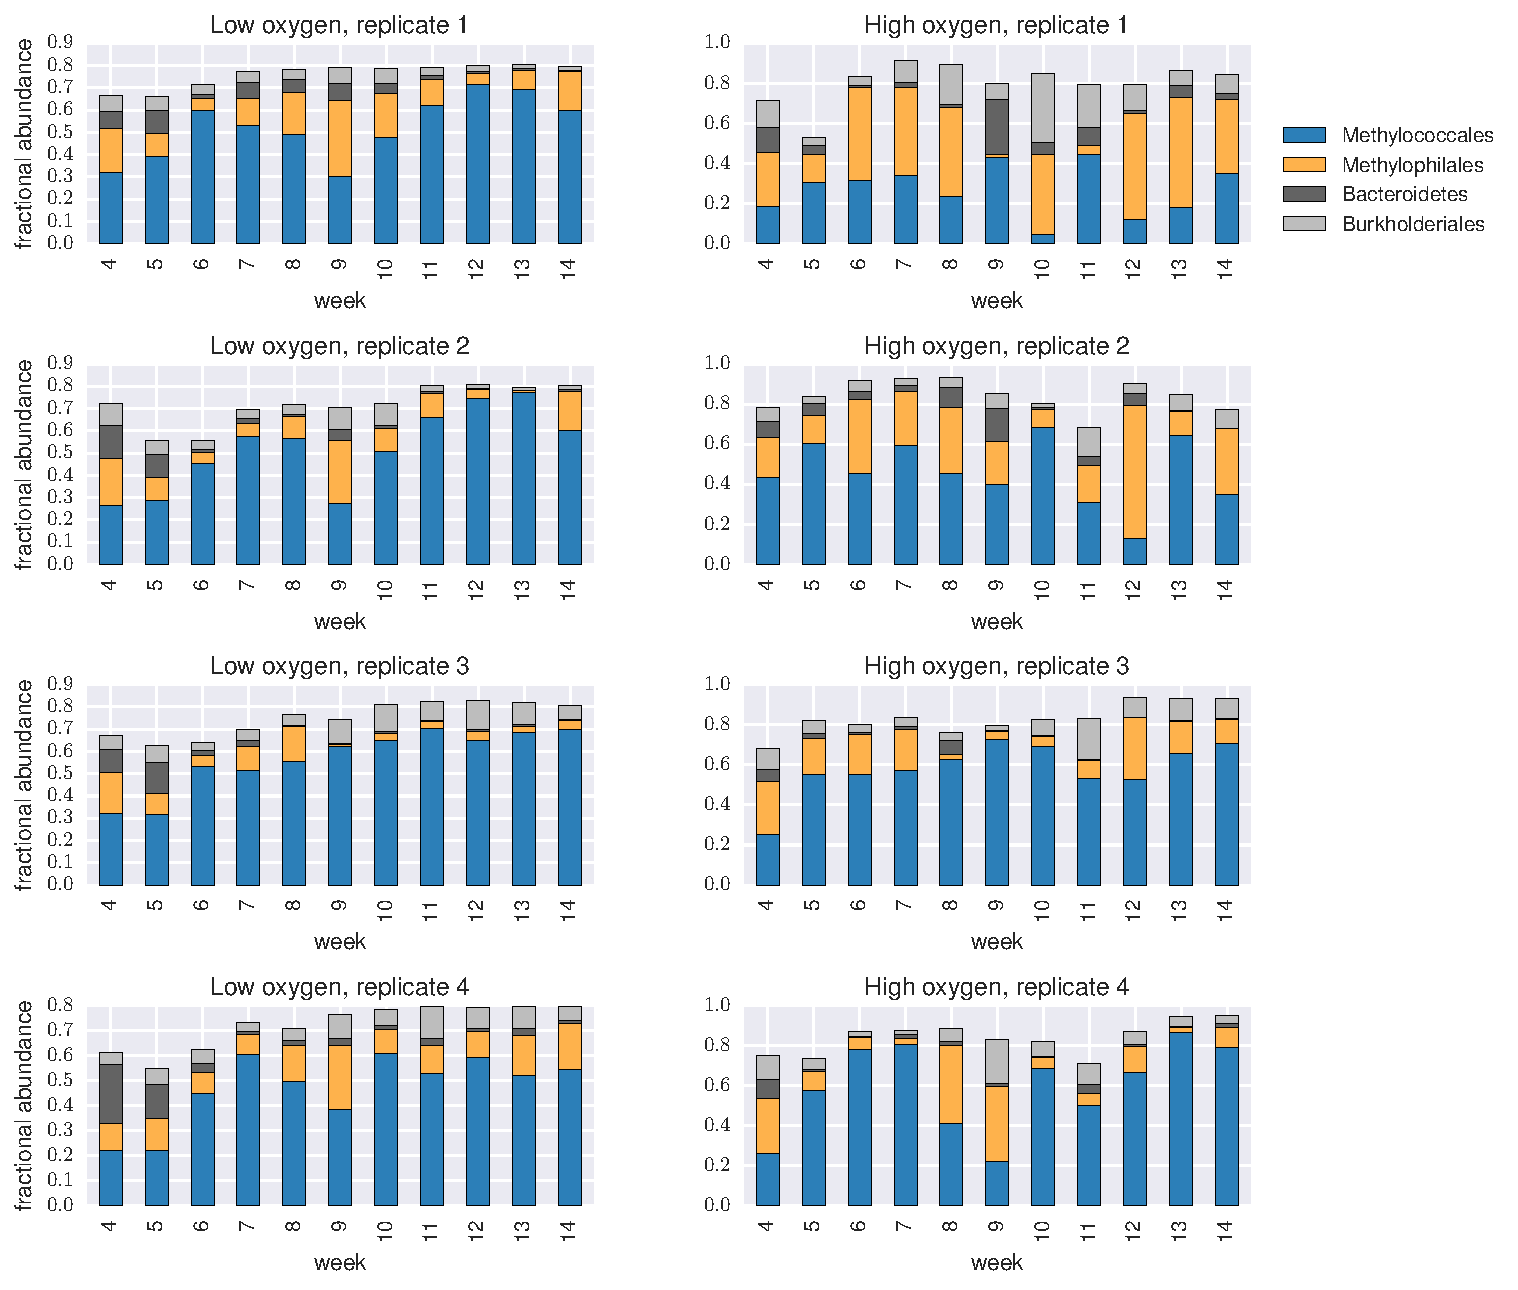
\includegraphics[width=1.0\textwidth]{./tex/chapter2/figures/170413_4_main_groups.pdf}  % ElvizAnalysis
    \begin{singlespace}
    \caption[Four major taxonomic groups in Lake Washington sediment incubations]{
        The abundance of the four major taxonomic groups in Lake Washington sediment incubations:
	Phylum Bacteroidetes, Orders Methylococcales (methylotrophs), Methylophilales (non-methanotrophic methylotrophs), Burkholderiales.}
    \label{fig:dominant_genera}
    \end{singlespace}
\end{figure}

\begin{figure}[H]
\centering
    % /Users/janet/elvizAnalysis/ipython_notebooks/plots/170313_methanotroph_methylotroph_taxa--portrait.pdf
    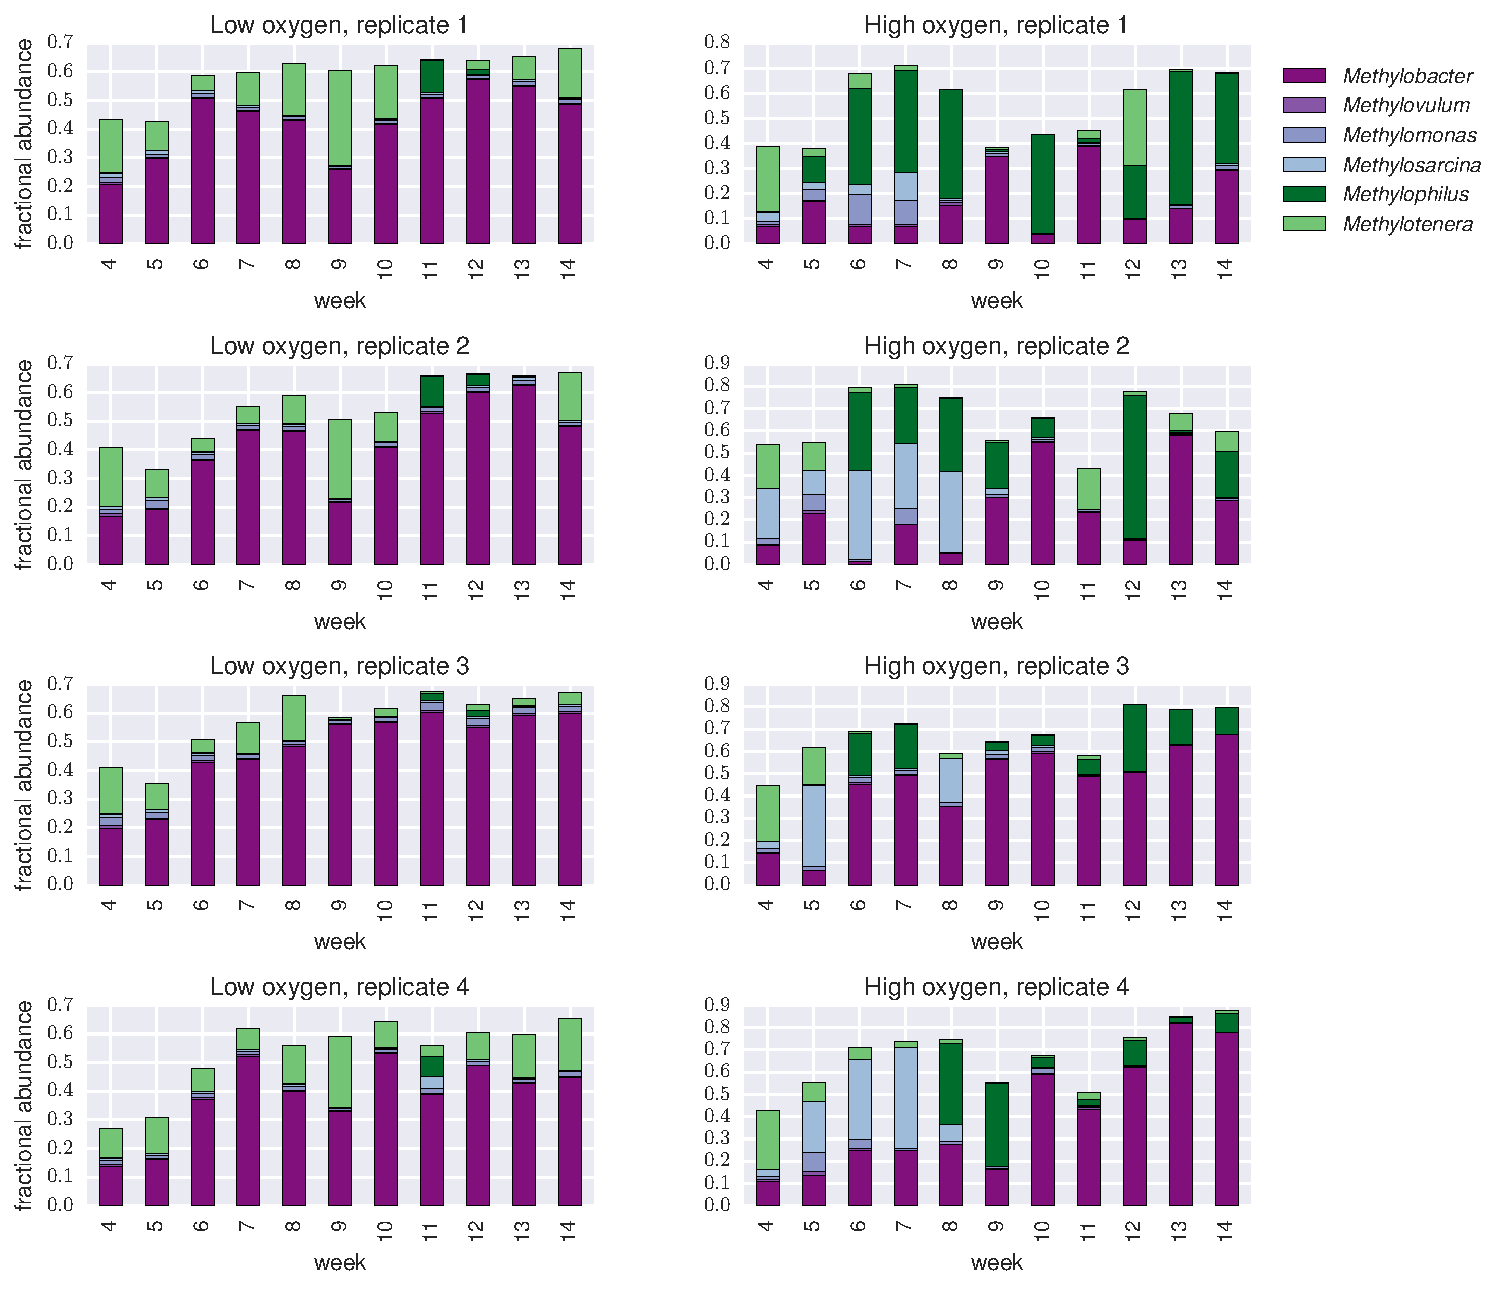
\includegraphics[width=1.0\textwidth]{./tex/chapter2/figures/170313_methanotroph_methylotroph_taxa--portrait.pdf}  % ElvizAnalysis
    \begin{singlespace}
    \caption[Dominant methanotrophic and methylotrophic Genera.]{
        Dominant methanotrophic (purples) and methylotrophic (greens) Genera.}
    \label{fig:dominant_genera}
    \end{singlespace}
\end{figure}

